\documentclass[12pt,ngerman,twoside]{scrartcl}
\usepackage{microtype}
\usepackage{lmodern}
%% Codelisting
%\usepackage{minted}
\usepackage{listings}

\lstset{
%numbers=left,
%numberstyle=\tiny,
%stepnumber=1,
%numbersep=8pt,
backgroundcolor=\color{lightgray},
frame=single,
basicstyle=\footnotesize,
breaklines=true,
commentstyle=\color{green}}

\usepackage{verbatim}				%kommentare

\usepackage[utf8]{inputenc}		%Encoding
\usepackage[T1]{fontenc}			%T1 Zeichensatz; Anführungszeichen usw.
\usepackage[scaled=0.92]{helvet}		%Schriftsatzklon Helvecia

%% Zeilenabstände 
\usepackage{setspace}
\onehalfspacing	

\usepackage[ngerman]{babel} 	%deutsche Rechtschreibung
\usepackage{ngerman}
\usepackage{parskip}				%Absatz wird nicht mehr eingerückt
\usepackage{hyperref}				%links

%% Packages für Grafiken & Abbildungen 
\usepackage{graphicx}
\usepackage[export]{adjustbox}  %Rahmen Bilder
\usepackage[font=small,labelfont=bf]{caption}
\captionsetup[figure]{font=small}
\newcommand{\source}[1]{\caption*{Quelle: {#1}}}
\usepackage{wrapfig}		%Fliesstext
\usepackage{subcaption}

%% Bibliograpy %%%%%%%%%%%%%%%%%%%%%%%%%%%%%%%%%%%%%%%%%%%%%%
%BEFINDET SICH IN LITERATURVERZEICHNIS
%\usepackage[style=apa,backend=biber]{biblatex}
%\DeclareLanguageMapping{ngerman}{ngerman-apa}
%\addbibresource{firefighterDocu.bib}

% IEEE
%\usepackage{natbib}
%\bibliography{firefighterDocu}

%Mathematische Symbole
\usepackage{mathtools}

%Abkürzungen
\usepackage[nohyperlinks, printonlyused, smaller]{acronym}

%Tabellen
\usepackage[table]{xcolor}

\definecolor{tableHeader}{RGB}{211, 47, 47}
\definecolor{tableLineOne}{RGB}{245, 245, 245}
\definecolor{tableLineTwo}{RGB}{224, 224, 224}

\usepackage{longtable}
\usepackage{multirow, varwidth}
\usepackage[table]{xcolor}


%Textersetzung
\newcommand{\base}{Steuer"=Server }
\newcommand{\internet}{Internetdienste"=Server }
\newcommand{\monitor}{Einsatzmonitor }
\newcommand{\push}{Browser"=Push"=Dienst }

\newcommand{\zcode}{ Zugangscode }

%Header
\usepackage{fancyhdr}


\begin{document}
\selectlanguage{ngerman}


\pagestyle{empty}
\KOMAoptions{twoside = false}

\begin{titlepage}
\centering
\begin{figure}[htbp]
\hspace*{3.3cm}
\end{figure}
        {\LARGE\bfseries BigData: Anwendungsresultate der verschiedenen Anwendungsmöglichkeiten von Hadoop \par}

\includegraphics[width=0.68\textwidth]{pics/hadoop.png}\par%
\vspace{0.1cm}
        Vorgelegt von: \\
        Huayi Sun 
        Martrikelnummer: 33338 \\ 
	e-Mail: huayi.juergens@studenten.hs-bremerhaven.de \\
        Daniel Paul Hoffmann 
        Martrikelnummer: 26355 \\
	e-Mail: daniel.hoffmann@studenten.hs-bremerhaven.de \\
        Michael Günster 
        Martrikelnummer: 32465 \\
	e-mail: michael.guenster@studenten.hs-bremerhaven.de \par

        Bearbeitungszeitraum: 22.03.2018 - 05.07.2018

% Bottom of the page
\vspace*{\fill}
{\small
        Modulverantwortliche: Prof. Dr. Nadija Syrjakow\par}
\end{titlepage}

\cleardoublepage

%\KOMAoptions{twoside = true}
\newpage
\tableofcontents				%Inhaltsverzeichnis
\newpage
\listoffigures 
\setcounter{page}{1}


%\pagestyle{headings}
\pagestyle{fancy}
\fancyhf{}
\fancyhead[LE]{\leftmark}
\fancyhead[RO]{\rightmark}
%\fancyfoot[CE,CO]{\leftmark}
\fancyfoot[LE,RO]{\thepage}


\newpage


\section{Umfrage: Mahout / Recommender (22.03.2018)}
\begin{itemize}
\item[-] Fragen Sie Ihre Kommilitonen nach Filmen,Getränken,Büchern,Musikvorlieben,etc.
\item[-] Lassen Sie obiges bewerten (1 bis 5 Sterne).
\item[-] Analysieren Sie die Umfrage mit Mahout Recommender
\end{itemize}

\subsection*{Kurzdarstellung der Aufgabenstellung}
Es soll eine Bewertungsumfrage bzgl. Büchern, Film o.Ä. getätigt werden. Hierbei sollen die Teilnehmer die jeweiligen Titel mit 1 bis 5 Sternen bewerten. Es ist hierbei von kritischer Bedeutung das kein Teilnehmer alle Titel/Objekt der Umfrage bewertet.

Die gesammelten Daten müssen entsprechend in Form einer .csv Datei aufbereitet werden für das anschließende Importieren in die Software. Nach dem Einlesen werden für einige Umfrageteilnehmer x Empfehlungen mit höchster Gefallenswahrscheinlichkeit abgefragt (abgeleitet aus den Bewertungen anderer Teilnehmer).

\subsection*{Lösung}
\begin{itemize}
\item[-] Visualisierung der getätigten Umfrage von 10 Teilnehmern zu 17 verschiedenen Filmen (\autoref{fig:recommender1}):
\begin{figure}[!htb]
        \begin{minipage}{1\textwidth}
                \centering
                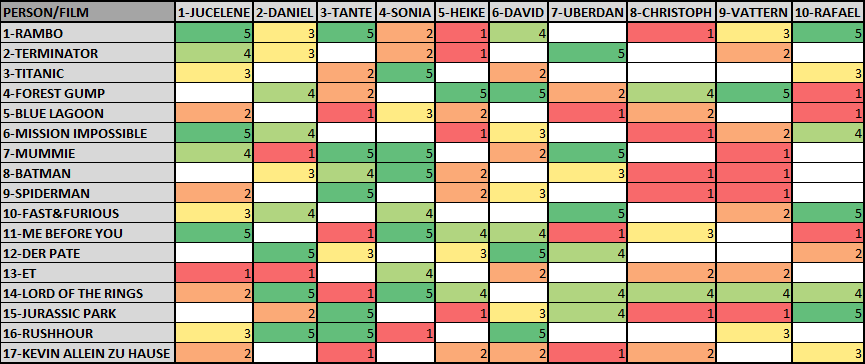
\includegraphics[width=0.90\textwidth]{pics/recommender1.png}\par\vspace{0cm}
                \caption{Tabelle: Umfrage}
                \label{fig:recommender1}
        \end{minipage}
\end{figure}

\item[-] Aufarbeitung Umfrage mit Excel für vorgegebenes Format: userID, itemId und prefValue (\autoref{fig:recommender2})
\begin{figure}[!htb]
        \begin{minipage}{1\textwidth}
                \centering
                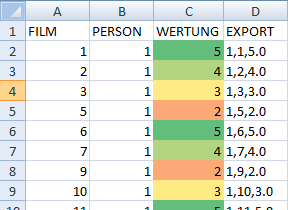
\includegraphics[width=0.40\textwidth]{pics/recommender2.png}\par\vspace{0cm}
                \caption{Tabelle: Aufarbeitung der Umfrage}
                \label{fig:recommender2}
        \end{minipage}
\end{figure}

\item[-] Starten Oracle 4.9 VM

\item[-] Kopieren der Daten aus Spalte D in eine Datei mit dem Namen „dataset.csv“ im Ordner /usr/temp/

\item[-] Oracle Jdeveloper starten

\item[-] Neues Java project angelegt: „myproject“ (gleicher Pfad Projekt)

\item[-] Bibliotheken aus den folgenden Ordnern hinzugefügt:
usr/lib/hadoop (all Libraries),
usr/lib/hadoop/lib (all Libraries),
usr/lib/Mahout/ (all Libraries),
usr/lib/Mahout/lib (all Libraries)

\item[-] Inhalt der recommender.txt Datei vom ELLI in das Java Projekt kopieren und den Filedatamodel und für die Emfpehlungsabfrage entsprechend die gewünschte Userid und Anzahl von Empfehlungen aufführen:
\end{itemize}

\begin{enumerate}
\item User 1 sollen nun 2 Filme empfohlen werden was zum Ergebnis in \autoref{fig:recommender3} führt:
\begin{figure}[!htb]
        \begin{minipage}{1\textwidth}
                \centering
                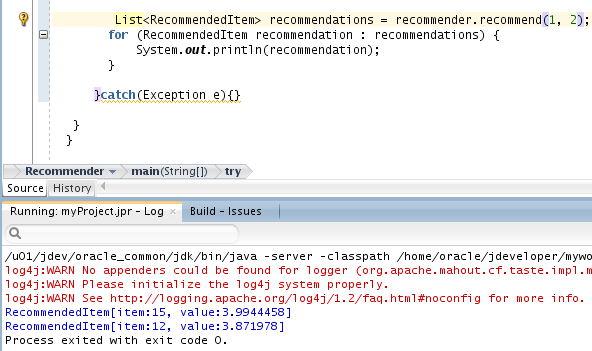
\includegraphics[width=0.90\textwidth]{pics/recommender3.png}\par\vspace{0cm}
                \caption{Tabelle: Ergebnis für User1}
                \label{fig:recommender3}
        \end{minipage}
\end{figure}

Es werden mit einer „Wahrscheinlichkeit des Gefallens“ von 3,87/5 bzw. 3,99/5   Userid 1 die Filme 12 („Der Pate“) und 15 („Jurassic Park“) empfohlen. Was augenscheinlich plausibel ist.

\item User 2 sollen nun 2 Filme empfohlen werden was zum Ergebnis in \autoref{fig:recommender4} führt:
\begin{figure}[!htb]
        \begin{minipage}{1\textwidth}
                \centering
                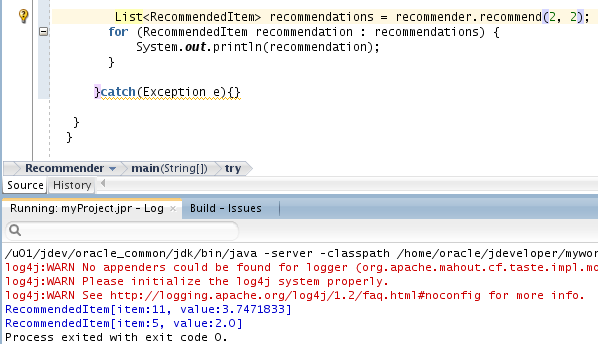
\includegraphics[width=0.90\textwidth]{pics/recommender4.png}\par\vspace{0cm}
                \caption{Tabelle: Ergebnis für User2}
                \label{fig:recommender4}
        \end{minipage}
\end{figure}

Es werden mit einer „Wahrscheinlichkeit des Gefallens“ von 3,75/5 bzw. 2/5 Userid 2 die Filme 11 („Me before You“) und 5 („Blue Lagoon“) empfohlen. Was augenscheinlich plausibel ist.

\item User 3 sollen nun 2 Filme empfohlen werden was zum Ergebnis in \autoref{fig:recommender5} führt:
\begin{figure}[!htb]
        \begin{minipage}{1\textwidth}
                \centering
                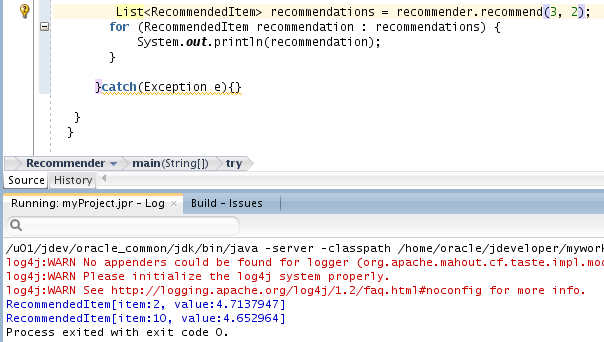
\includegraphics[width=0.90\textwidth]{pics/recommender5.png}\par\vspace{0cm}
                \caption{Tabelle: Ergebnis für User3}
                \label{fig:recommender5}
        \end{minipage}
\end{figure}


Es werden mit einer ''Wahrscheinlichkeit des Gefallens`` von 4,71/5 bzw. 4,65/5 Userid 2 die Filme 10 (``Me before You``) und 5 (``Fast \& Furious``) empfohlen. Was augenscheinlich plausibel ist.

\end{enumerate}

\subsection*{Aufteilung der Aufgaben im Team}
\subsection*{Darstellung der benutzen Werkzeuge und Systeme}
\subsubsection*{Entwurfswerkzeug}
Microsoft Excel
\subsubsection*{Entwicklungsumgebung}
JDeveloper




\newpage


\section{12.04.2018 - PIG}
Führen Sie folgende Pig Operationen mit Ihren Testdaten (Bags) aus: LOAD,  Dump, Join, Cross, Union, Split

\subsection{Kurzdarstellung der Aufgabenstellung}
Datensätze in From von .csv Datein in HDFS Ordner Laden und Mittels PIG die im HDFS bereitgestellten Datensätze auswerten. Der grundlegende Umgang mit Daten in PIG als Bestandteil von HADOOP soll durch bereitstellen von Daten in HDFS und das abfragen/analysieren in PIG selbiger geprobt werden.
\subsection{Lösung}
- Starten der Oracle 4.9 VM

Ändern von Tastaturlayout auf DE mittels Terminaleingabe:
\begin{lstlisting}
setxkbmap -layout de
\end{lstlisting}

Anlegen eines eigenes Ordners für die Aufgabenstellung auf der VM:
\begin{lstlisting}
mkdir /usr/tmp/gruppe
\end{lstlisting}

Drei Textdateien (artikel, ek\_pos\_1, ek\_pos\_2) in /usr/tmp/gruppe/ mit Testdaten anlegen:
\begin{figure}[!htb]
        \begin{minipage}{1\textwidth}
                \centering
                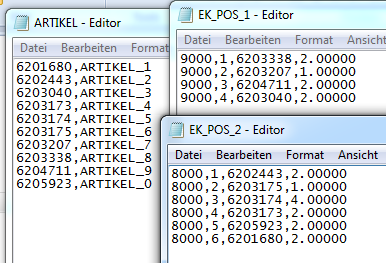
\includegraphics[width=0.90\textwidth]{pics/pig1.png}\par\vspace{0cm}
                \caption{Tabellen}
                \label{fig:pig1}
        \end{minipage}
\end{figure}

Über den Termin einen HDFS Ordner fuer die Aufgabenstellung anlegen:
\begin{lstlisting}
hdfs dfs -mkdir hdfs://bigdatalite.localdomain:8020/tmp/gruppe
\end{lstlisting}

Zuvor angelegte Textdatei in usr/tmp/gruppe in HDFS Ordner (.../tmp/gruppe) kopieren:
\begin{lstlisting}
hdfs dfs -put /usr/tmp/gruppe/ek_pos_1 hdfs://bigdatalite.localdomain:8020/tmp/gruppe
hdfs dfs -put /usr/tmp/gruppe/ek_pos_2 hdfs://bigdatalite.localdomain:8020/tmp/gruppe
hdfs dfs -put /usr/tmp/gruppe/artikel hdfs://bigdatalite.localdomain:8020/tmp/gruppe
\end{lstlisting}

Show files on datastore (printscreen Ergebnis):
\begin{lstlisting}
hdfs dfs -ls /tmp/gruppe
\end{lstlisting}

Start Pig
\begin{lstlisting}
pig -x mapreduce
\end{lstlisting}

Verlassen der Shell: 
\begin{lstlisting}
exit the Grunt shell using 'ctrl + d'
\end{lstlisting}


Daten aus HDFS Ordner in PIG laden, unter angabe der Spaltennamen und Datentypen:
\begin{lstlisting}
artikel = LOAD 'hdfs://bigdatalite.localdomain:8020/tmp/gruppe/artikel' USING
PigStorage(',') as (art_id:int, art_name:chararray);

ek_pos_1 = LOAD 'hdfs://bigdatalite.localdomain:8020/tmp/gruppe/ek_pos_1'       USING    PigStorage(',') as (kd_id:int, pos:int, art_id:int, menge:int);

ek_pos_2 = LOAD 'hdfs://bigdatalite.localdomain:8020/tmp/gruppe/ek_pos_2'       USING PigStorage(',') as (kd_id:int, pos:int, art_id:int, menge:int);
\end{lstlisting}

Ausführen von Abfragen auf den und deren Ausgaben:

\subsubsection*{UNION}
\begin{lstlisting}
ek_positionen = UNION ek_pos_1, ek_pos_2;
dump ek_positionen;
--(8000,1,6202443,2)
--(8000,2,6203175,1)
--(8000,3,6203174,4)
--(8000,4,6203173,2)
--(8000,5,6205923,2)
--(8000,6,6201680,2)
--(9000,1,6203338,2)
--(9000,2,6203207,1)
--(9000,3,6204711,2)
--(9000,4,6203040,2)
\end{lstlisting}

\subsubsection*{JOIN}
\begin{lstlisting}
ek_art_join = JOIN ek_positionen by art_id,artikel by art_id;
dump ek_art_join;
--(8000,6,6201680,2,6201680,ARTIKEL_1)
--(8000,1,6202443,2,6202443,ARTIKEL_2)
--(9000,4,6203040,2,6203040,ARTIKEL_3)
--(8000,4,6203173,2,6203173,ARTIKEL_4)
--(8000,3,6203174,4,6203174,ARTIKEL_5)
--(8000,2,6203175,1,6203175,ARTIKEL_6)
--(9000,2,6203207,1,6203207,ARTIKEL_7)
--(9000,1,6203338,2,6203338,ARTIKEL_8)
--(9000,3,6204711,2,6204711,ARTIKEL_9)
--(8000,5,6205923,2,6205923,ARTIKEL_0)
\end{lstlisting}

\subsubsection*{SPLIT}
\begin{lstlisting}
SPLIT ek_pos_1 into einkauf_1_1 if pos<3, einkauf_1_2 if pos>2;
dump einkauf_1_1;
--(9000,1,6203338,2)
--(9000,2,6203207,1)

dump einkauf_1_2; (Ausgabe fehlt)
\end{lstlisting}


\subsubsection*{CROSS}
\begin{lstlisting}
ek_pos_cross = CROSS ek_pos_1, ek_pos_2;
dump ek_pos_cross;
--(9000,4,6203040,2,8000,6,6201680,2)
--(9000,4,6203040,2,8000,5,6205923,2)
--(9000,4,6203040,2,8000,4,6203173,2)
--(9000,4,6203040,2,8000,3,6203174,4)
--(9000,4,6203040,2,8000,2,6203175,1)
--(9000,4,6203040,2,8000,1,6202443,2)
--(9000,3,6204711,2,8000,6,6201680,2)
--(9000,3,6204711,2,8000,5,6205923,2)
--(9000,3,6204711,2,8000,4,6203173,2)
--(9000,3,6204711,2,8000,3,6203174,4)
--(9000,3,6204711,2,8000,2,6203175,1)
--(9000,3,6204711,2,8000,1,6202443,2)
--(9000,2,6203207,1,8000,6,6201680,2)
--(9000,2,6203207,1,8000,5,6205923,2)
--(9000,2,6203207,1,8000,4,6203173,2)
--(9000,2,6203207,1,8000,3,6203174,4)
--(9000,2,6203207,1,8000,2,6203175,1)
--(9000,2,6203207,1,8000,1,6202443,2)
--(9000,1,6203338,2,8000,6,6201680,2)
--(9000,1,6203338,2,8000,5,6205923,2)
--(9000,1,6203338,2,8000,4,6203173,2)
--(9000,1,6203338,2,8000,3,6203174,4)
--(9000,1,6203338,2,8000,2,6203175,1)
--(9000,1,6203338,2,8000,1,6202443,2)
\end{lstlisting}

\subsection{Aufteilung der Aufgaben im Team}
\subsection{Darstellung der benutzen Werkzeuge und Systeme}
\subsubsection*{Entwurfswerkzeug}
\subsubsection*{Entwicklungsumgebung}





\newpage


\section{Hbase (03.05.2018)}
\begin{itemize}
\item[-] Erzeugen Sie für Ihr Beispiel 2 Hbase (Shell) Tabellen.
\item[-] Füllen Sie die Tabellen mit einigen Testdaten.
\item[-] (Java API) Erzeugen Sie für Ihr Beispiel zwei Hbase Tabellen.
\item[-] Füllen Sie die Tabellen mit einigen Testdaten.
\item[-] Listen Sie die Tabellen auf.
\end{itemize}
\subsection*{Kurzdarstellung der Aufgabenstellung}
Zum Einstieg in NoSQL Datenbanken sollen in Apache Hbase je zwei Tabellen mittels Shell Interface und Java-Code? erstellt und mit Daten befüllt werden. Weiterhin sollen die angelegten Tabellen in Hbase ausgegeben werden mittels vorgegebenen Java-Code.
\subsection*{Lösung}

\begin{itemize}
\item[-] Oracle VM 4.9 starten

\item[-] Tastatur auf Deutsch stellen mittels Eingabe Befehl in Terminal:
\begin{lstlisting}
setxkbmap -layout de
\end{lstlisting}

\subsubsection*{HBASE}
\item[-] HBASE über folgenden Befehlt im Terminal der VM starten:
\begin{lstlisting}
hbase shell
\end{lstlisting}

\item[-] Anlegen der Tabelle „companies“ mit den attributen „id“ und „property“
\begin{lstlisting}
create 'companies1', 'id', 'property'
\end{lstlisting}

\item[-] Daten in die zuvor angelegte Tabelle „companies1“ schreiben:
\begin{lstlisting}
put 'companies1', 'row1', 'id:HRNR', '162'
put 'companies1', 'row1', 'property:Name', 'Musterfirma'
put 'companies1', 'row1', 'property:Gruendung', '1979'
\end{lstlisting}

\item[-] Tabelle „companies1“ mit geschriebenen Daten ausgeben lassen:
\begin{lstlisting}
get 'companies1', 'row1'

COLUMN                CELL
id:HRNR              timestamp=1529566648268, value=162
property:Gruendung   timestamp=1529566667304, value=1979
property:Name        timestamp=1529566659389, value=Musterfirma
3 row(s) in 0.0400 seconds
\end{lstlisting}

\item[-] Anlegen der Tabelle „products1“ mit den attributen „id“ und „property“
\begin{lstlisting}
 create 'products1', 'id', 'property'
\end{lstlisting}

\item[-] Daten in die zuvor angelegte Tabelle „products1“ schreiben:
\begin{lstlisting}
put 'products1', 'row1', 'id:ISBN10', '3866471769'
put 'products1', 'row1', 'id:ISBN13', '978-3866471764'
put 'products1', 'row1', 'property:Typ', 'Buch'
put 'products1', 'row1', 'property:Titel', 'Krieg und Frieden'
put 'products1', 'row1', 'property:Seitenanzahl', '1536'
\end{lstlisting}

\item[-] Tabelle „products1“ mit geschriebenen Daten ausgeben lassen:
\begin{lstlisting}
get 'products1', 'row1'
COLUMN                CELL
id:ISBN10            timestamp=1529566771386, value=3866471769
id:ISBN13            timestamp=1529566777916, value=978-3866471764
property:Seitenanzah timestamp=1529566805924, value=1536
property:Titel       timestamp=1529566797799, value=Krieg und Frieden
property:Typ         timestamp=1529566790781, value=Buch

5 row(s) in 0.0220 seconds
\end{lstlisting}

\subsubsection*{Mittels Java-API}
In der Oracle VM verifizieren ob HBASE als Service gestartet ist und ggf. starten.
\item[-]Oracle JDeveloper 12c starten und Java Developer auswählen
\item[-]Java Projekt „A0305“ mit gewünschtem Zielpfad anlegen „/usr/tmp/dph/A0305/“
\item[-]Alle Java Klassen zu A0305 durch Rechtsklick auf Projektnamen hinzufügen aus:
Location : usr/lib/hadoop (all Library)
Location : usr/lib/hadoop/lib (all Library)
Location : usr/lib/hbase (all Library)
Location : usr/lib/hbase/lib (all Library)
\item[-] Übernahme und Ausführung der SCRIPTE aus den Materialien (Korrektur: TableDescriptor in HtableDescriptor)

\item[-]Anlegen Tabelle „companies2“ mit Spalten „id“ und „property“ (\autoref{fig:hbase1})
\begin{figure}[!htb]
        \begin{minipage}{1\textwidth}
                \centering
                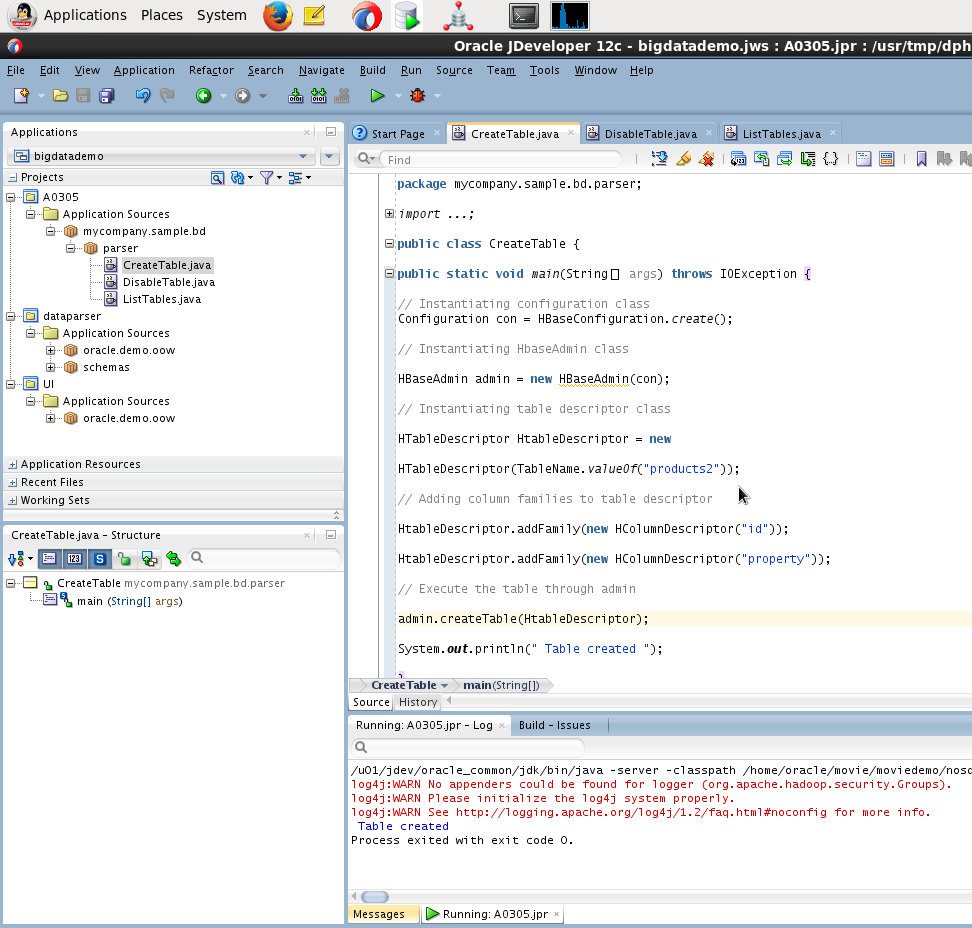
\includegraphics[width=0.90\textwidth]{pics/hbase1.png}\par\vspace{0cm}
                \caption{Tabelle: companies2}
                \label{fig:hbase1}
        \end{minipage}
\end{figure}

\item[-] Anlegen Tabelle „products2“ mit Spalten „id“ und „property“(\autoref{fig:hbase2})
\begin{figure}[!htb]
        \begin{minipage}{1\textwidth}
                \centering
                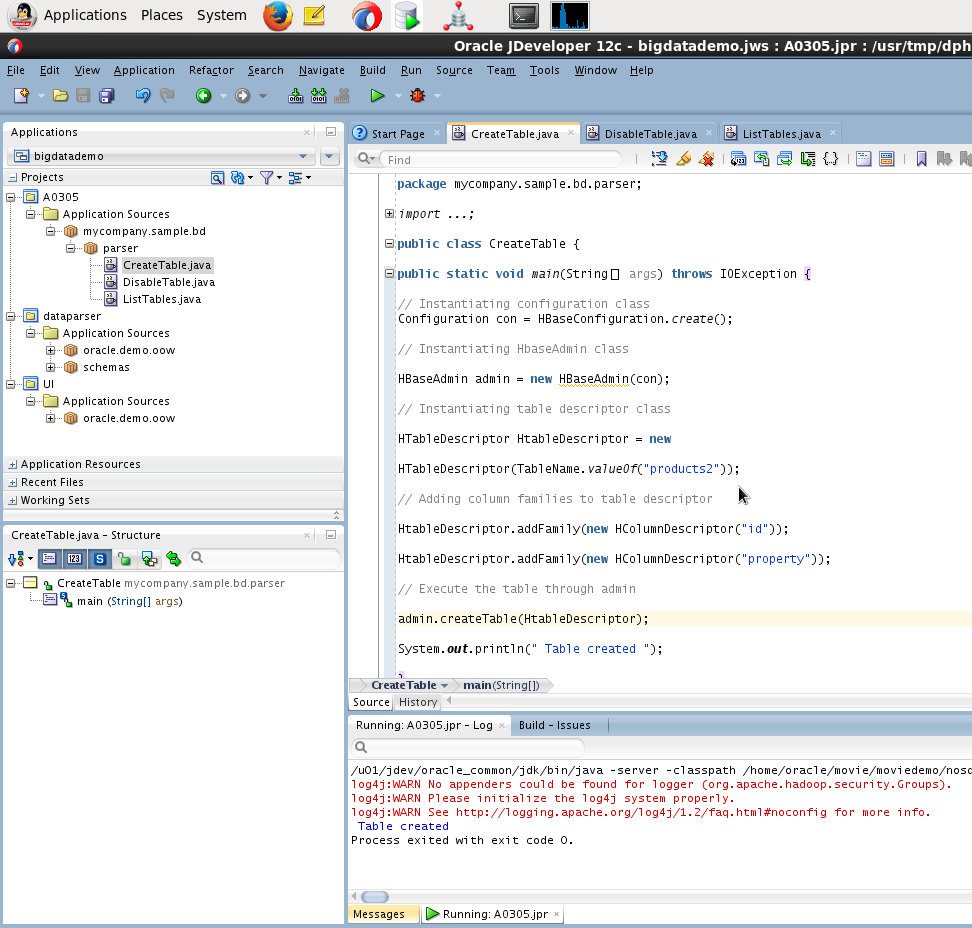
\includegraphics[width=0.90\textwidth]{pics/hbase2.png}\par\vspace{0cm}
                \caption{Tabelle: products2}
                \label{fig:hbase2}
        \end{minipage}
\end{figure}

\item[-] Ausgabe aller angelegten Tabellen in HBASE mittels vorgebenem JAVA code(\autoref{fig:hbase3}):
\begin{figure}[!htb]
        \begin{minipage}{1\textwidth}
                \centering
                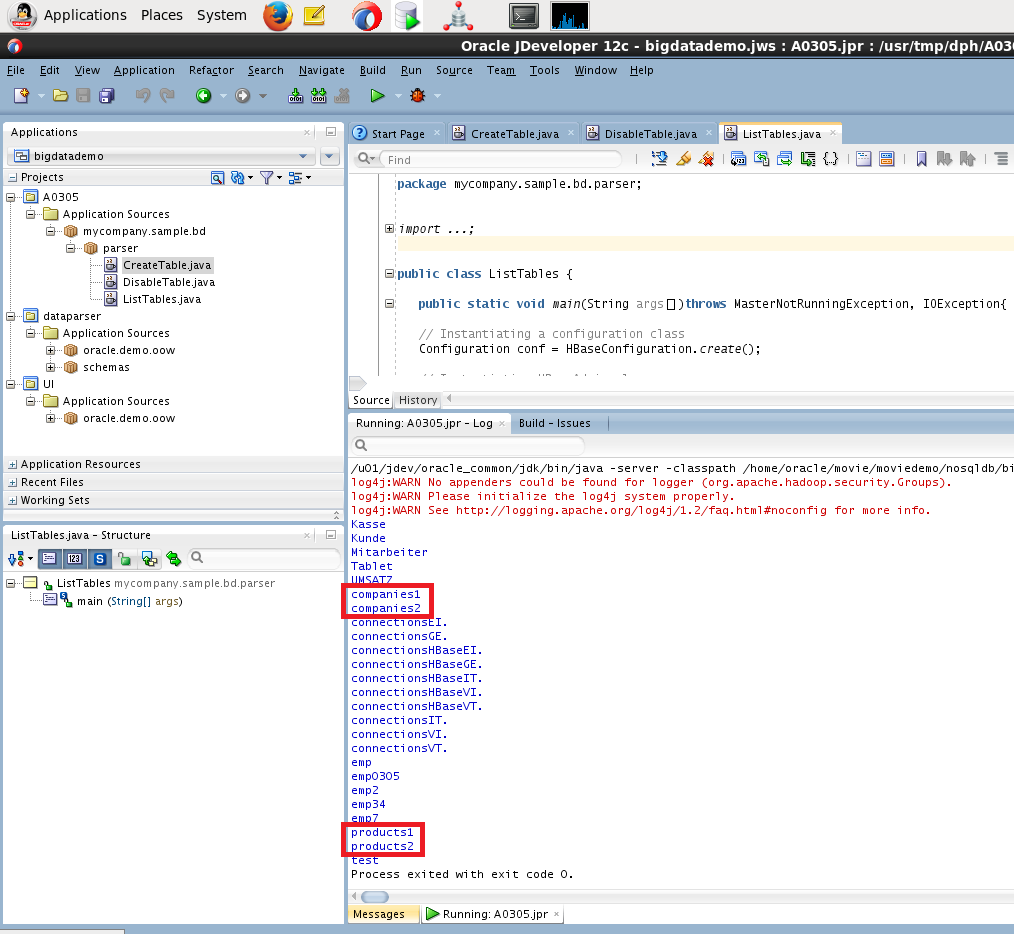
\includegraphics[width=0.90\textwidth]{pics/hbase3.png}\par\vspace{0cm}
                \caption{Ausgabe aller Tabellen}
                \label{fig:hbase3}
        \end{minipage}
\end{figure}

\item[-] Hbase ueber den Terminal der Oracle VM starten:
\begin{lstlisting}
hbase shell
\end{lstlisting}

\item[-] Daten in die zuvor angelegte Tabelle „companies2“ schreiben:
\begin{lstlisting}
put 'companies2', 'row1', 'id:HRNR', '976'
put 'companies2', 'row1', 'property:Name', 'TheRealDeal'
put 'companies2', 'row1', 'property:Gruender', 'Mr. X'
put 'companies2', 'row1', 'property:Employees', '35'
\end{lstlisting}

\item[-] Tabelle „companies2“ mit geschriebenen Daten ausgeben lassen:
\begin{lstlisting}
get 'companies2', 'row1'
COLUMN                CELL
id:HRNR              timestamp=1529567187758, value=976
property:Employees   timestamp=1529567210676, value=35
property:Gruender    timestamp=1529567203411, value=Mr. X
property:Name        timestamp=1529567196336, value=TheRealDeal
4 row(s) in 0.0290 seconds
\end{lstlisting}

\item[-] Daten in die zuvor angelegte Tabelle „products2“ schreiben:
\begin{lstlisting}
put 'products2', 'row1', 'id:ASIN', 'B015XI6BWE'
put 'products2', 'row1', 'id:Herstellernr', '20B7S1C600'
put 'products2', 'row1', 'id:EAN', '4260444483708'
put 'products2', 'row1', 'property:Typ', 'Laptop'
put 'products2', 'row1', 'property:Model', 'T440'
put 'products2', 'row1', 'property:Marke', 'Think Pad'
0 row(s) in 0.0140 seconds
\end{lstlisting}

\item[-] Tabelle „companies1“ mit geschriebenen Daten ausgeben lassen:
\begin{lstlisting}
get 'products2', 'row1'
COLUMN                CELL
id:ASIN              timestamp=1529567272010, value=B015XI6BWE
id:EAN               timestamp=1529567286841, value=4260444483708
id:Herstellernr      timestamp=1529567279612, value=20B7S1C600
property:Marke       timestamp=1529567306209, value=Think Pad
property:Model       timestamp=1529567299462, value=T440
property:Typ         timestamp=1529567293694, value=Laptop
6 row(s) in 0.0380 seconds
\end{lstlisting}
\end{itemize}
\subsection*{Aufteilung der Aufgaben im Team}
Alle Punkte wurden gemeinsam bearbeitet.
\subsection*{Darstellung der benutzen Werkzeuge und Systeme}

\subsubsection*{Entwurfswerkzeug}
JDeveloper/HBASE
\subsubsection*{Entwicklungsumgebung}
HBASE



\newpage


\section{R Turotium (17.05.2018, 24.05.2018) }
\begin{itemize}
\item[-]Führen Sie die im Tutorium: https://www.tutorialspoint.com/r/r\_web\_data.htm angegebenen Unterpunkte zu R Data Interfaces, R Charts \& Graphs und R Statistics Examples aus.
\item[-]Wenden Sie anschließend die Beispiele aus den Tutorien auf Ihre eigenen Daten an
\end{itemize}

\subsection*{Kurzdarstellung der Aufgabenstellung}
Es soll die grundlegende Funktionsweise von R verstanden werden durch die Anwendung oeffentlich zugänglicher Tutorials.

\subsection*{Lösung}
Als Dataset wurde die Bevoelkerungshistorie der einzelnen EU Laender nach Jahren zwischen 1960 und 2016 gewaehlt. 

\begin{itemize}
\item[-]Zuerst wird R-Studio gestartet

\item[-]Mittels folgendem Befehl ermittelt wir das working directory auf die R-Installation eingestellt ist(\autoref{fig:tutor1}):
\begin{figure}[!htb]
        \begin{minipage}{1\textwidth}
                \centering
                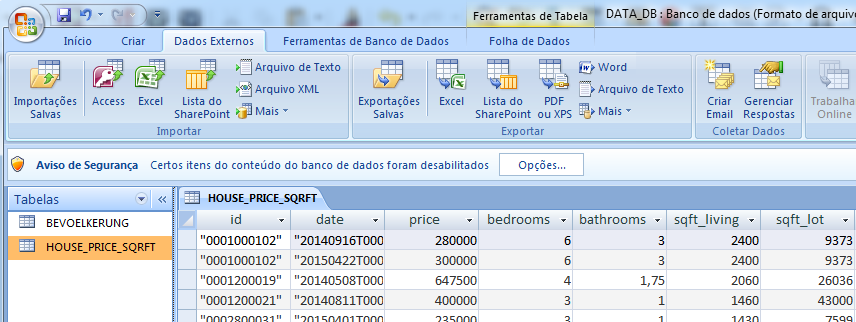
\includegraphics[width=0.50\textwidth]{pics/tutor1.png}\par\vspace{0cm}
                \caption{Standardpfad festlegen}
                \label{fig:tutor1}
        \end{minipage}
\end{figure}
	
\item[-]Die .csv Datei („BEVOELKERUNG.csv“)wird in den zuvor ermittelten Ordner gelegt

\item[-]Über den folgenden Befehl werden die Daten aus \\ „C:/Users/admin/Documents/BEVOELKERUNGSDATEN.csv“ in eine R variable geladen:
\begin{lstlisting}
data <- read.csv("BEVOELKERUNG.csv")
\end{lstlisting}
\item[-]Über diesen Befehl werden die ersten 6 Zeilen einer Variable ausgegeben werden(\autoref{fig:tutor2}):
\begin{figure}[!htb]
        \begin{minipage}{1\textwidth}
                \centering
                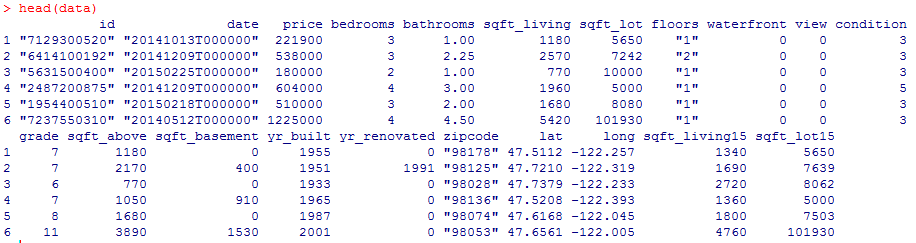
\includegraphics[width=0.50\textwidth]{pics/tutor2.png}\par\vspace{0cm}
                \caption{Anzeige der Zeilen}
                \label{fig:tutor2}
        \end{minipage}
\end{figure}

\section*{Tortendiagramm}
Zum Vergleich der Bevoelkerungsverteilung ueber die Laender der heutigen EU soll je ein Torten-Diagramm für 1996 und 2016 erstellt werden:

\subsection*{1966}
\item[-]Daten für 1966 muessen zuerst ein eine Variable separiert werden:
\begin{lstlisting}
J1966 <- data[ which(data$Jahr==1966), ]
\end{lstlisting}
\item[-]Ausgabe der ersten 6 Zeilen von J1966(\autoref{fig:tutor3}):
\begin{figure}[!htb]
        \begin{minipage}{1\textwidth}
                \centering
                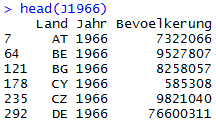
\includegraphics[width=0.50\textwidth]{pics/tutor3.png}\par\vspace{0cm}
                \caption{Ausgabe Variable}
                \label{fig:tutor3}
        \end{minipage}
\end{figure}

\item[-]Zum Erstellen des Diagramm werden zuerst die betreffenden Spalten in Variablen verwiesen mittels der folgenden beiden Befehle:
\begin{lstlisting}
x <- J1966$Bevoelkerung
labels <- J1966$Land
\end{lstlisting}
\item[-]Dateiname und Typ für die Diagramm-Ausgabe festlegen:
\begin{lstlisting}
png(file = "Bevoelkerung_1966.jpg")
\end{lstlisting}
			
\item[-]Plotten des Diagramms
\begin{lstlisting}
pie(x,labels, main = "Bevoelkerung 1966")
\end{lstlisting}

\item[-]Diagramm in zuvor angebene Datei ``Bevoelkerung\_1996.jpg`` speichern:
\begin{lstlisting}
dev.off()
\end{lstlisting}

\item[-]Fertiges Diagramm(\autoref{fig:tutor4}):
\begin{figure}[!htb]
        \begin{minipage}{1\textwidth}
                \centering
                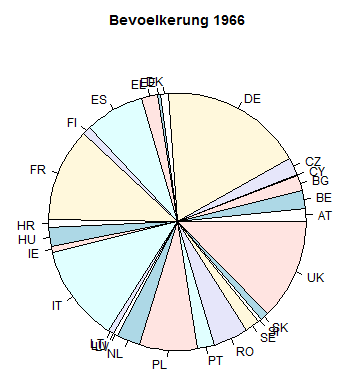
\includegraphics[width=0.50\textwidth]{pics/tutor4.png}\par\vspace{0cm}
                \caption{Bevölkerung 1966}
                \label{fig:tutor4}
        \end{minipage}
\end{figure}

\section*{2016}
\item[-]Daten für 2016 muessen zuerst ein eine Variable separiert werden:
\begin{lstlisting}
J2016 <- data[ which(data$Jahr==2016), ]		
\end{lstlisting}
		
\item[-]Ausgabe der ersten 6 Zeilen von J2016(\autoref{fig:tutor5}):
\begin{figure}[!htb]
        \begin{minipage}{1\textwidth}
                \centering
                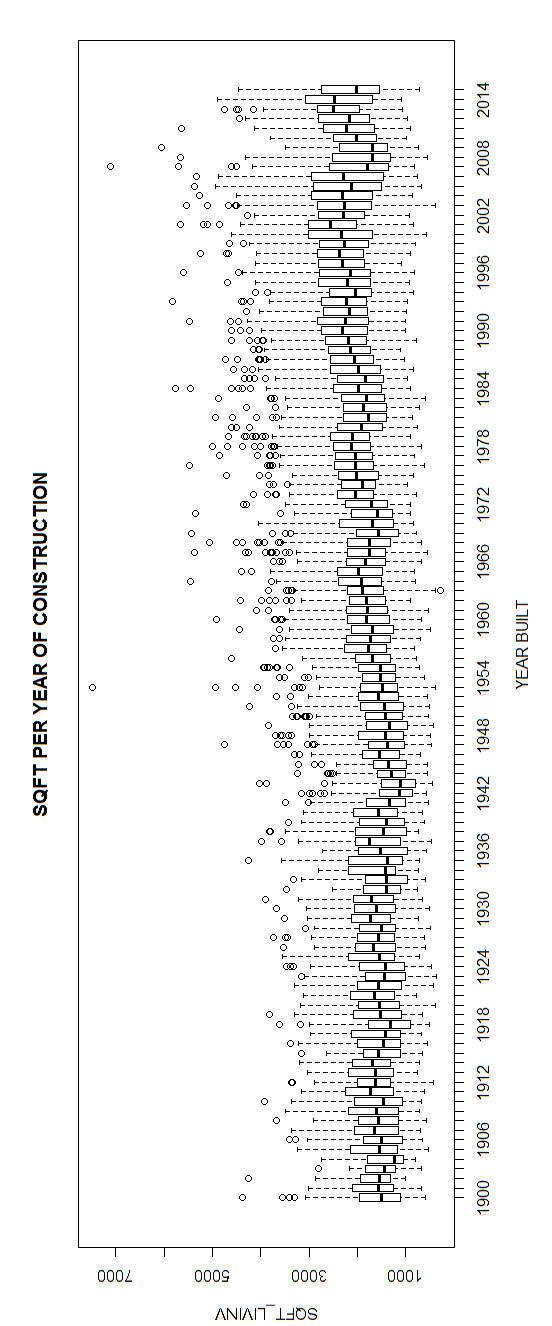
\includegraphics[width=0.50\textwidth]{pics/tutor5.png}\par\vspace{0cm}
                \caption{Variablenausgabe}
                \label{fig:tutor5}
        \end{minipage}
\end{figure}
\item[-]Zum Erstellen des Diagramm werden zuerst die betreffenden Spalten in Variablen verwiesen mittels der folgenden beiden Befehle:
\begin{lstlisting}
x <- J2016$Bevoelkerung
labels <- J2016$Land
\end{lstlisting}
\item[-]Dateiname und Typ für die Diagramm-Ausgabe festlegen:
\begin{lstlisting}
png(file = "Bevoelkerung_2016.jpg")
\end{lstlisting}
\item[-]Plotten des Diagramms
\begin{lstlisting}
pie(x,labels, main = "Bevoelkerung 2016")
\end{lstlisting}
\item[-]Diagramm in zuvor angebene Datei ``Bevoelkerung\_2016.jpg`` speichern:
\begin{lstlisting}
dev.off()
\end{lstlisting}
\item[-]fertiges Diagramm(\autoref{fig:tutor6}):
\begin{figure}[!htb]
        \begin{minipage}{1\textwidth}
                \centering
                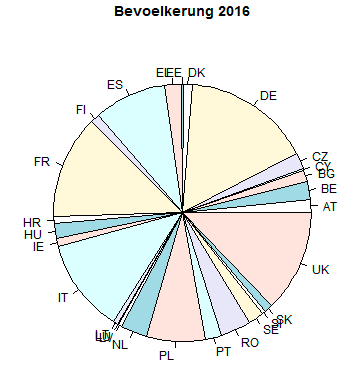
\includegraphics[width=0.50\textwidth]{pics/tutor6.png}\par\vspace{0cm}
                \caption{Bevölerung 2016}
                \label{fig:tutor6}
        \end{minipage}
\end{figure}

\section*{Bar-Charts}
\subsection*{Frankreich}
\item[-]Daten für Frankreich muessen zuerst ein eine Variable separiert werden:
\begin{lstlisting}
FR <- data[ which(data$Land=='FR'), ]
\end{lstlisting}
\item[-]Ausgabe der ersten 6 Zeilen von FR(\autoref{fig:tutor7}):
\begin{figure}[!htb]
        \begin{minipage}{1\textwidth}
                \centering
                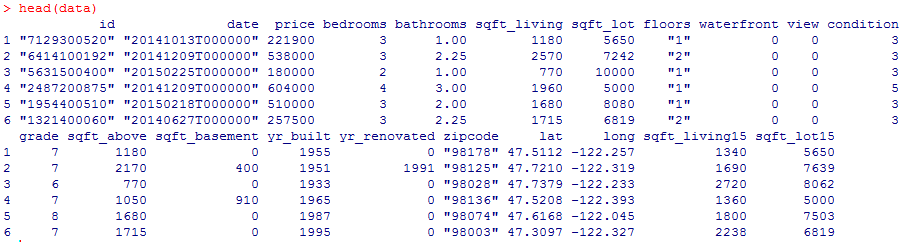
\includegraphics[width=0.50\textwidth]{pics/tutor7.png}\par\vspace{0cm}
                \caption{Zeilenausgabe}
                \label{fig:tutor7}
        \end{minipage}
\end{figure}
\item[-]Zum Erstellen des Diagramm werden zuerst die betreffenden Spalten in Variablen verwiesen mittels der folgenden beiden Befehle:
\begin{lstlisting}
Y <- FR$Bevoelkerung
X <- FR$Jahr
\end{lstlisting}
\item[-]Dateiname und Typ für die Diagramm-Ausgabe festlegen:
\begin{lstlisting}
png(file = "Bevoelkerunghistorie_Frankreich.png")
\end{lstlisting}
\item[-]Plotten des Diagramms
\begin{lstlisting}
barplot(Y,names.arg=X,xlab="Jahr",ylab="Bevoelkerung",col="blue",main="Bevoelkerungsentwicklung FR")
\end{lstlisting}
\item[-]Diagramm in zuvor angebene Datei ``Bevoelkerung\_2016.jpg`` speichern:
\begin{lstlisting}
dev.off()
\end{lstlisting}
\item[-]fertiges Diagramm(\autoref{fig:tutor8}):

\begin{figure}[!htb]
        \begin{minipage}{1\textwidth}
                \centering
                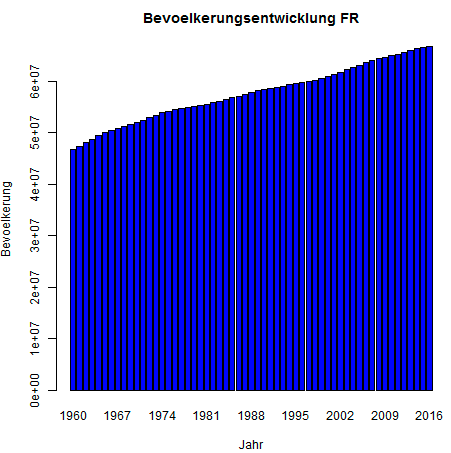
\includegraphics[width=0.50\textwidth]{pics/tutor8.png}\par\vspace{0cm}
                \caption{Diagramm: Frankreich}
                \label{fig:tutor8}
        \end{minipage}
\end{figure}

\section*{Deutschland}
\item[-]Daten für Deutschland muessen zuerst ein eine Variable separiert werden:
\begin{lstlisting}
DE <- data[ which(data$Land=='DE'), ]
\end{lstlisting}
\item[-]Ausgabe der ersten 6 Zeilen von de(\autoref{fig:tutor9}):
\begin{figure}[!htb]
        \begin{minipage}{1\textwidth}
                \centering
                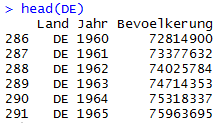
\includegraphics[width=0.50\textwidth]{pics/tutor9.png}\par\vspace{0cm}
                \caption{Variablenverwendung}
                \label{fig:tutor9}
        \end{minipage}
\end{figure}
\item[-]Zum Erstellen des Diagramm werden zuerst die betreffenden Spalten in Variablen verwiesen mittels der folgenden beiden Befehle:
\begin{lstlisting}
Y <- DE$Bevoelkerung
X <- DE$Jahr
\end{lstlisting}

\item[-]Dateiname und Typ für die Diagramm-Ausgabe festlegen:
\begin{lstlisting}
png(file = "Bevoelkerunghistorie_Deutschland.png")
\end{lstlisting}
\item[-]Plotten des Diagramms
\begin{lstlisting}
barplot(Y,names.arg=X,xlab="Jahr",ylab="Bevoelkerung",col="blue",main="Bevoelkerungsentwicklung DE")
\end{lstlisting}
\item[-]Diagramm in zuvor angebene Datei ``Bevoelkerung\_2016.jpg`` speichern:
\begin{lstlisting}
dev.off()
\end{lstlisting}
\item[-]fertiges Diagramm(\autoref{fig:tutor10}):
\begin{figure}[!htb]
        \begin{minipage}{1\textwidth}
                \centering
                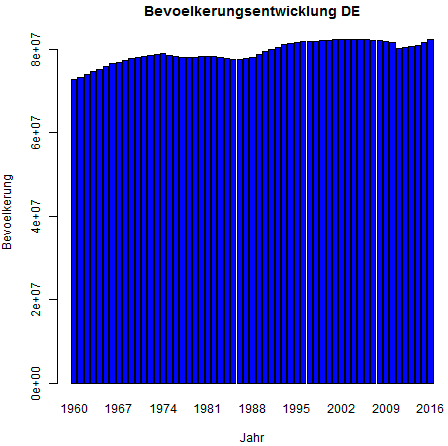
\includegraphics[width=0.50\textwidth]{pics/tutor10.png}\par\vspace{0cm}
                \caption{Bevölkerungsentwicklung DE}
                \label{fig:tutor10}
        \end{minipage}
\end{figure}
\subsection*{Statistik für R-Tutorium => NEUER ABSATZ}
\item[-]Auswertung des Mittelwertes (mean) und der Summe (sum) Bevölkerung EU 1966
\begin{lstlisting}
	print(mean(J1966$Bevoelkerung))
	print(sum(J1966$Bevoelkerung))
\end{lstlisting}

\item[-]Auswertung des Mittelwertes (mean) und der Summe (sum) Bevölkerung EU 2016
\begin{lstlisting}
	print(mean(J2016$Bevoelkerung))
	print(sum(J2016$Bevoelkerung))
\end{lstlisting}

\end{itemize}
\subsection*{Aufteilung der Aufgaben im Team}
Alle Aufgabenpunkte wurden gemeinsam bearbeitet.
\subsection*{Darstellung der benutzen Werkzeuge und Systeme}
\subsubsection*{Entwurfswerkzeug}
R-Studio
\subsubsection*{Entwicklungsumgebung}
R-Studio



\newpage

\section{R RJDBC / Access (31.05.2018) }
\begin{itemize}
\item[-]Suchen Sie sich einen für Sie interessanten Bereich aus bspw. Marktforschung, soziale Netzwerke, Wetterstationen, Gesundheitswesen, Natur und Sozialwissenschaften, etc.
\item[-]Führen Sie einen Tabellen Entwurf durch.
\item[-]Erzeugen Sie die Tabellen (Oracle Datenbank).
\item[-]Füllen Sie die Tabellen mit einigen Testdaten
\item[-]Bauen Sie eine RJDBC Verbindung (R) zur Oracle Datenbank auf.
\item[-]Analysieren Sie die Daten
\item[-]Suchen Sie in deren Datenbeständen nach unbekannten Zusammenhängen.
\end{itemize}
\subsection*{Kurzdarstellung der Aufgabenstellung}
Es sollen Daten aus einem beliegen Bereich gewählt werden und in einer Datenbank abgelegt werden. Auf die Datenbank soll mit R zugriffen werden um die Daten analysieren zu können.
\subsection*{Lösung}
\begin{itemize}
\item[-]Gewählter Datensatz: https://www.kaggle.com/harlfoxem/housesalesprediction beinhaltet Hausverkaufsdaten von Häusern in King County (USA) im Jahre 2014
\item[-]Daten wurden in MS-Access (C:/users/admin/documents/DATA\_DB.mdb) mit der CSV-Importfunktion eingelesen(\autoref{fig:rjdbc1})
\begin{figure}[!htb]
        \begin{minipage}{1\textwidth}
                \centering
                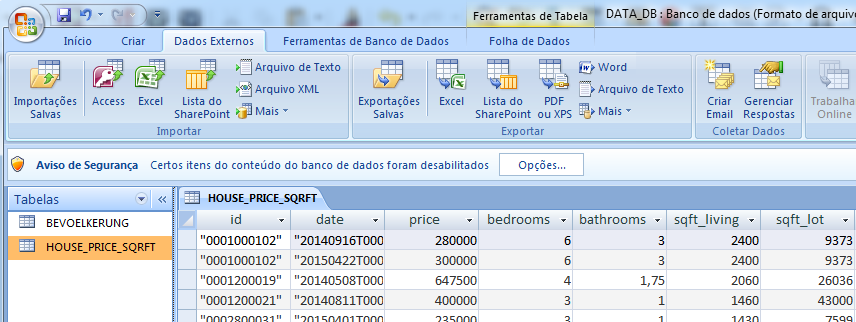
\includegraphics[width=0.90\textwidth]{pics/rjdbc1.png}\par\vspace{0cm}
                \caption{Import MS-Access}
                \label{fig:rjdbc1}
        \end{minipage}
\end{figure}

Für die Analyse wurde nur R gestartet und folgende Aktionen/Befehle ausgeführt:
\item[-]Installieren RODBC Package:
\begin{lstlisting}
install.packages("RODBC")
\end{lstlisting}
\item[-]Aufrufen Package RODBC:
\begin{lstlisting}
library(RODBC)
\end{lstlisting}
\item[-]Zuweisen Genutzten Datenbank auf (abgelegt in R source Ordner)
\begin{lstlisting}
channel <- odbcConnectAccess("DATA_DB.mdb")
\end{lstlisting}

\item[-]Zweisen der Datentabelle auf Objekt:
\begin{lstlisting}
data = sqlQuery(channel ,paste('SELECT * FROM HOUSE_PRICE_SQRFT'))
\end{lstlisting}

\item[-]Anzeigen der ersten sechs Zeilen der Tabelle/Objekt(\autoref{fig:rjdbc2})
\begin{figure}[!htb]
        \begin{minipage}{1\textwidth}
                \centering
                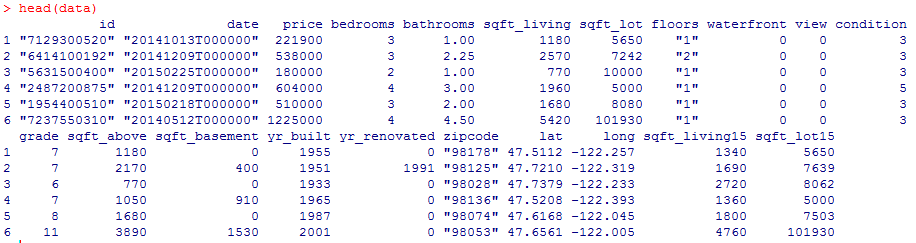
\includegraphics[width=0.90\textwidth]{pics/rjdbc2.png}\par\vspace{0cm}
                \caption{Anzeigen der Zeilen}
                \label{fig:rjdbc2}
        \end{minipage}
\end{figure}

\item[-]Analyse Histogram Preis(\autoref{fig:rjdbc3}):
\begin{lstlisting}
hist(data$price,xlab = "price",col = "green",border = "red"
\end{lstlisting}

\begin{figure}[!htb]
        \begin{minipage}{1\textwidth}
                \centering
                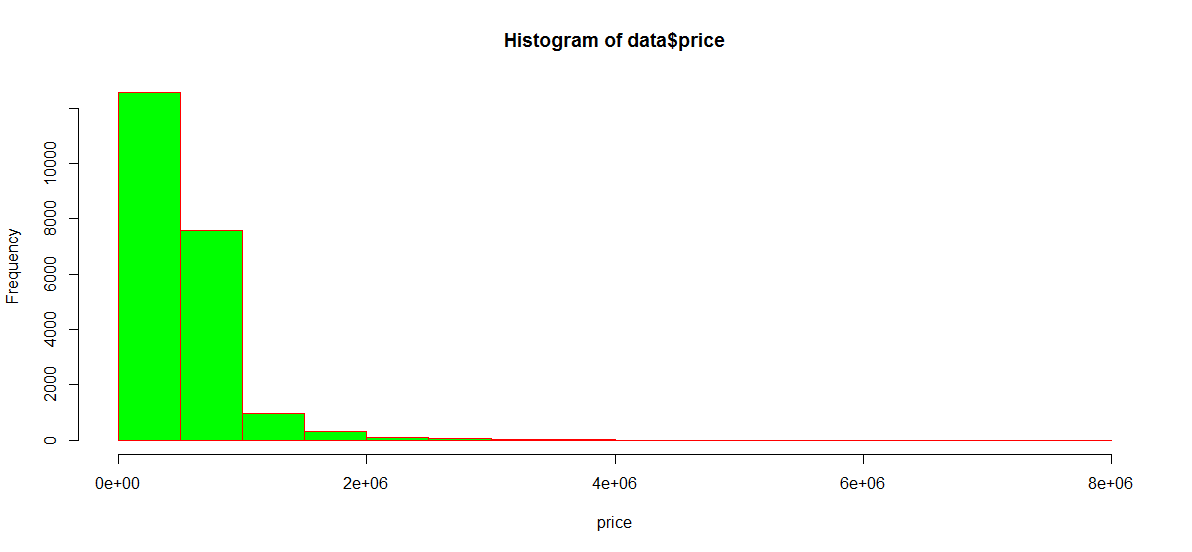
\includegraphics[width=0.90\textwidth]{pics/rjdbc3.png}\par\vspace{0cm}
                \caption{Analyse Histogramm}
                \label{fig:rjdbc3}
        \end{minipage}
\end{figure}

\item[-]Datensatz auf Preise bis maximal 1mio reduzieren:
\begin{lstlisting}
data = sqlQuery(channel ,paste('SELECT * FROM HOUSE_PRICE_SQRFT WHERE PRICE < 1000001'))
\end{lstlisting}

\item[-]Neues Histogramm ausführen(\autoref{fig:rjdbc4}):
\begin{lstlisting}
hist(data$price,xlab = "price",col = "green",border = "red")
\end{lstlisting}

\begin{figure}[!htb]
        \begin{minipage}{1\textwidth}
                \centering
                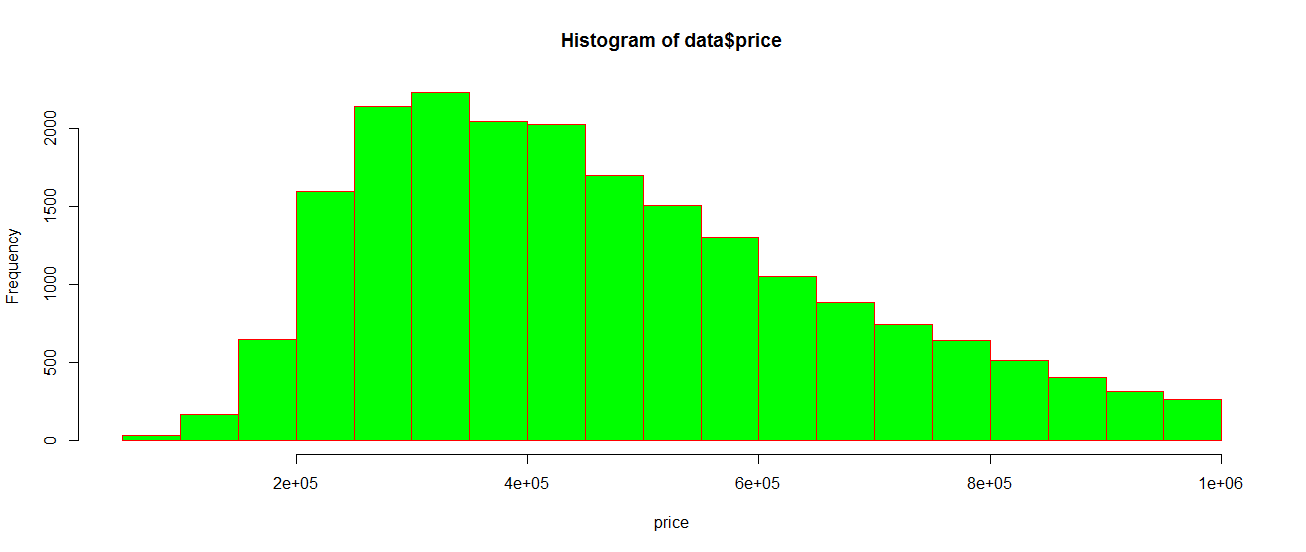
\includegraphics[width=0.90\textwidth]{pics/rjdbc4.png}\par\vspace{0cm}
                \caption{Weiteres Histogramm}
                \label{fig:rjdbc4}
        \end{minipage}
\end{figure}

\item[-]Abfrage minimum Preis in der Datei(\autoref{fig:rjdbc4-1}):
\begin{figure}[!htb]
        \begin{minipage}{1\textwidth}
                \centering
                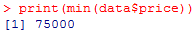
\includegraphics[width=0.50\textwidth]{pics/rjdbc4-1.png}\par\vspace{0cm}
                \caption{Abfrage Preis}
                \label{fig:rjdbc4-1}
        \end{minipage}
\end{figure}

\item[-]Boxplot (Wohnraufgrößen Variation pro Baujahr)(\autoref{fig:rjdbc5}):
\begin{lstlisting}
boxplot(sqft_living ~ yr_built, data = data, xlab = "YEAR BUILT",+    ylab = "SQFT_LIVINV", main = "SQFT PER YEAR OF CONSTRUCTION")
\end{lstlisting}

\begin{figure}[!htb]
        \begin{minipage}{1\textwidth}
                \centering
                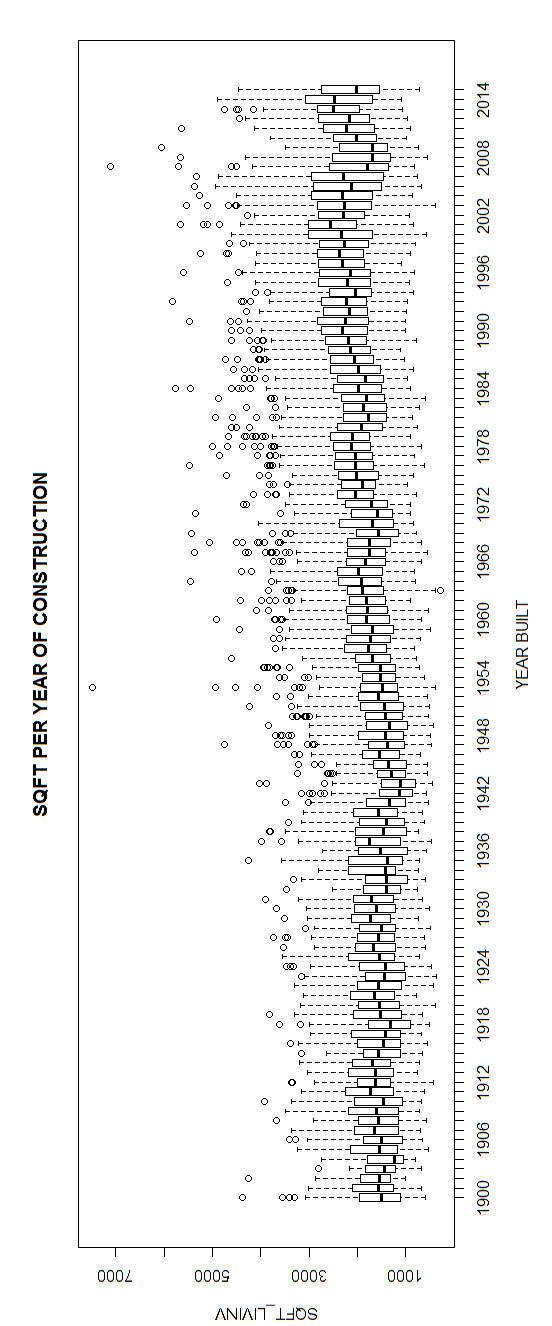
\includegraphics[width=0.50\textwidth]{pics/rjdbc5.png}\par\vspace{0cm}
                \caption{Boxplot SQFT per year of construction}
                \label{fig:rjdbc5}
        \end{minipage}
\end{figure}

\item[-]Erstellen von SCATTER PLOT MATRIX(\autoref{fig:rjdbc6}):
\begin{lstlisting}
pairs(~price+sqft_living+sqft_lot,data = data,  +    main = "Scatterplot Matrix")
\end{lstlisting}

\begin{figure}[!htb]
        \begin{minipage}{1\textwidth}
                \centering
                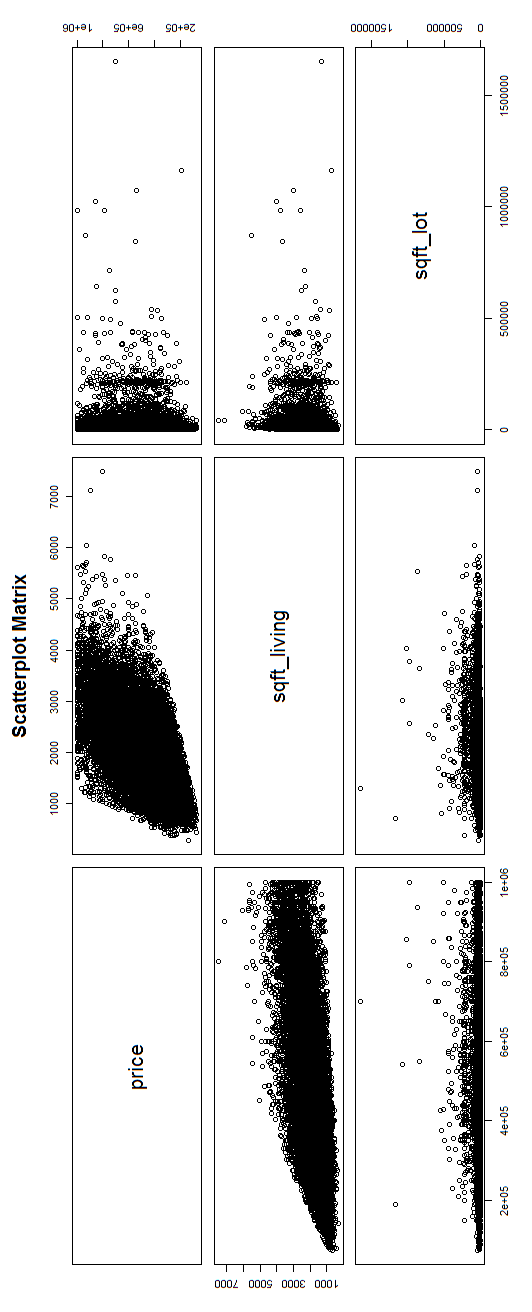
\includegraphics[width=0.50\textwidth]{pics/rjdbc6.png}\par\vspace{0cm}
                \caption{Scatterplot}
                \label{fig:rjdbc6}
        \end{minipage}
\end{figure}

\item[-]multiple lineare Regression (Price in Abängigkeit Sqft\_Living und Sqft\_Loft)

\item[-]Installation und Öffnung der relevanten Daten
\begin{lstlisting}
install.packages("caret")
install.packages("ggplot2")
install.packages("lattice")
library(caret)
\end{lstlisting}

\item[-]Verwendung der Daten in der variable „data“(\autoref{fig:rjdbc7})

\begin{figure}[!htb]
        \begin{minipage}{1\textwidth}
                \centering
                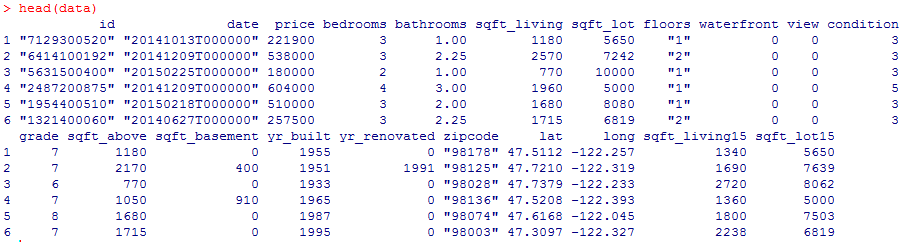
\includegraphics[width=0.90\textwidth]{pics/rjdbc7.png}\par\vspace{0cm}
                \caption{Variablenverwendung}
                \label{fig:rjdbc7}
        \end{minipage}
\end{figure}

\item[-]Verwendung Modell für multiple lineare Regression mit allen mathematisch        vorstellbar relevanten spalten
\begin{lstlisting}
model <-lm(price~bedrooms+bathrooms+sqft_living+sqft_lot+waterfront+    view+condition+grade+sqft_above+sqft_basement+yr_built+yr_renovated,    data = data)
\end{lstlisting}

\item[-]Ausgabe des berechneten Modells(\autoref{fig:rjdbc8}):
\begin{figure}[!htb]
        \begin{minipage}{1\textwidth}
                \centering
                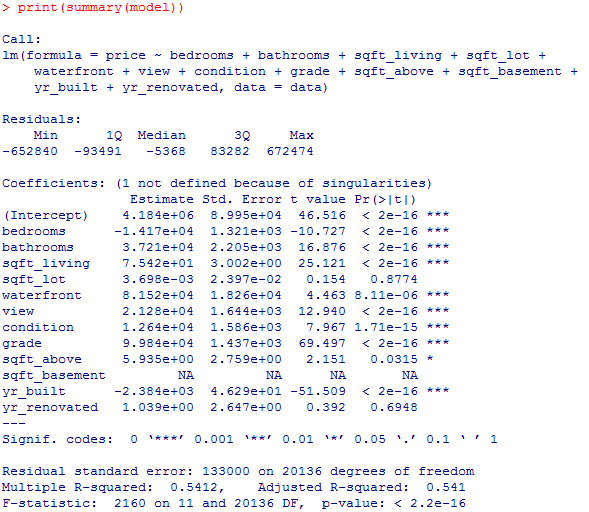
\includegraphics[width=0.60\textwidth]{pics/rjdbc8.png}\par\vspace{0cm}
                \caption{Ausgabe Berechnungsmodell}
                \label{fig:rjdbc8}
        \end{minipage}
\end{figure}
\end{itemize}
\subsection*{Aufteilung der Aufgaben im Team}
Alle Aufgabenpunkte wurden gemeinsam bearbeitet
\subsection*{Darstellung der benutzen Werkzeuge und Systeme}
\subsubsection*{Entwurfswerkzeug}
MS-ACCESS, Textdatei(csv)
\subsubsection*{Entwicklungsumgebung}
R (32bit Version da MS-ACCESS 32bit Version ansonsten Verbindung in der Form nicht möglich)



\newpage
\section{R / Hive (07.06.2018)}
\begin{itemize}
\item[-] Suchen Sie sich einen für Sie interessanten Bereich aus bspw. Marktforschung, soziale Netzwerke, Wetterstationen, Gesundheitswesen, Natur und Sozialwissenschaften, etc.
\item[-] Erzeugen Sie für Ihr Beispiel zwei Hive Tabellen
\item[-] Füllen Sie die Tabellen mit einigen Testdaten (LOAD DATA, Insert).
\item[-] Bauen Sie eine R Verbindung zur HIVE auf.
\item[-] Analysieren Sie die Daten
\end{itemize}
\subsection*{Kurzdarstellung der Aufgabenstellung}
Mittels dem Anlegen von zwei Tabellen in HIVE und dem anschließenden Bearbeiten/Analysieren mit R soll die das Zusammenspiel von relevanter Software für BigData geübt/demonstriert werden.
\subsection*{Lösung}
\subsubsection*{HIVE}
\begin{itemize}
\item[-] Ordner in /usr/tmp/hive/ anlegen
\item[-] Datensets „hotels.csv“ und „autos.csv“  in /usr/tmp/hive/ legen
\item[-] HIVE über den Terminal in Oracle VM4.9:

\begin{lstlisting}
hive
\end{lstlisting}

\item[-] Separate Datenbank im HIVE anlegen, falls keine namentlich identische existiert und verwenden:
\begin{lstlisting}
CREATE DATABASE IF NOT EXISTS diim18;
use diim18;
\end{lstlisting}

\item[-] Tabelle „hotels“ anlegen mit folgendem Befehl:
\begin{lstlisting}
Create TABLE hotels(gewinn FLOAT, preisInMio FLOAT,qm FLOAT,stadt String) ROW Format DELIMITED FIELDS Terminated by ',' Lines terminated by '\n';
\end{lstlisting}

\item[-] Tabelle „autos“ anlegen mit folgendem Befehl:
\begin{lstlisting}
Create TABLE autos(preis FLOAT, registrierungJahr INT,ps FLOAT,km INT,  modell String, kraftstoff STRING, name STRING) ROW Format DELIMITED FIELDS      Terminated by ',' Lines terminated by '\n';
\end{lstlisting}

\item[-] Daten aus hotels.csv in HIVE Tabelle hotels laden:
\begin{lstlisting}
LOAD DATA LOCAL INPATH '/usr/tmp/hive/hotels/hotels.csv' Overwrite INTO Table hotels;
\end{lstlisting}

\item[-] Daten aus hotels.csv in HIVE Tabelle hotels laden:
\begin{lstlisting}
LOAD DATA LOCAL INPATH '/usr/tmp/hive/autos/autos.csv' Overwrite INTO Table autos;
\end{lstlisting}
\item[-] Ausgabe der angelegten Tabellen.(\autoref{fig:hive1})
\begin{figure}[!htb]
        \begin{minipage}{1\textwidth}
                \centering
                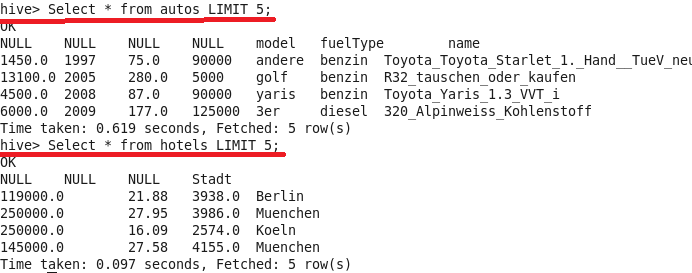
\includegraphics[width=0.90\textwidth]{pics/HIVE.png}\par\vspace{0cm}
                \caption{Ausgabe Tabellen}
                \label{fig:hive1}
        \end{minipage}
\end{figure}
Die Daten können nun mit SQL Statements betrachtet und manipuliert werden

\subsubsection*{R}
\item[-]Starten von R durch Eingabe in den terminal auf der Oracle 4.9 VM:
\begin{lstlisting}
R
\end{lstlisting}

\item[-] Installieren des RJDBC packages:
\begin{lstlisting}
install.packages("RJDBC",dep=TRUE)
\end{lstlisting}

\item[-] Aufrufen des RJDBC packages:
\begin{lstlisting}
library("RJDBC")
\end{lstlisting}

\item[-] Driver auf variable in R zur Verwendung zuweisen:
\begin{lstlisting}
drv <-JDBC("org.apache.hive.jdbc.HiveDriver","/usr/lib/hive/lib         /hive-jdbc.jar")
\end{lstlisting}

\item[-] Connection Type hinzufügen:

\begin{lstlisting}
library("ORCH")
ore.connect(type="HIVE")
ore.sync()
\end{lstlisting}

\item[-] Verbindung zu R aufbauen
\begin{lstlisting}
conn <- dbConnect(drv, "jdbc:hive2://localhost:10000/diim18", "", "")
\end{lstlisting}

\item[-] Inhalt der Tabelle autos im Hive auf die Variable autos in R zuweisen:
\begin{lstlisting}
autos <- dbGetQuery(conn, "Select * from autos")
\end{lstlisting}

\item[-] Lineares Regressionsmodell (lRm) erstellen: autos.preis = a * autos.km + b
\begin{lstlisting}
model <-lm(autos.preis~autos.km, data = autos)
\end{lstlisting}

\item[-] Modell Zusammenfassung ausgeben lassen (\autoref{fig:hive2}):
\begin{figure}[!htb]
        \begin{minipage}{1\textwidth}
                \centering
                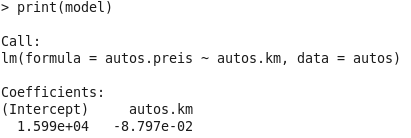
\includegraphics[width=0.60\textwidth]{pics/autos_model_1.png}\par\vspace{0cm}
                \caption{Ausgabe: model}
                \label{fig:hive2}
        \end{minipage}
\end{figure}


\item[-] Erstellen einer neuen Spalte in Autos die den Preis auf Basis des lRm:
\begin{lstlisting}
autos$predicted_1 <- predict(model, autos)
\end{lstlisting}

\item[-] multiples Rm (mRm) erstellen: autos.preis = a * autos.km + b * autos.ps + b
\begin{lstlisting}
model <-lm(autos.preis~autos.km+autos.ps, data = autos)
\end{lstlisting}

\item[-] Modell Zusammenfassung ausgeben lassen (\autoref{fig:hive3}):
\begin{figure}[!htb]
        \begin{minipage}{1\textwidth}
                \centering
                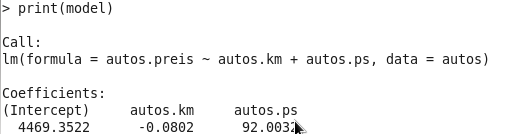
\includegraphics[width=0.60\textwidth]{pics/autos_model_2.png}\par\vspace{0cm}
                \caption{Ausgabe: model}
                \label{fig:hive3}
        \end{minipage}
\end{figure}


\item[-] Erstellen einer neuen Spalte in Autos die den Preis auf Basis des mRm (\autoref{fig:hive4})
\begin{lstlisting}
autos$predicted_2 <- predict(model, autos)
print(model)
head(autos)
\end{lstlisting}
\begin{figure}[!htb]
        \begin{minipage}{1\textwidth}
                \centering
                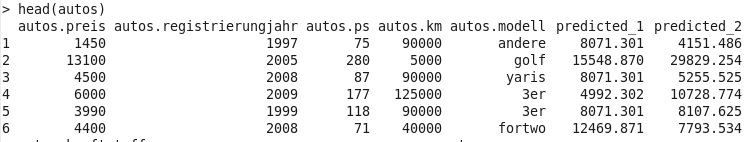
\includegraphics[width=0.70\textwidth]{pics/autos_head.png}\par\vspace{0cm}
                \caption{Ausgabe: autos}
                \label{fig:hive4}
        \end{minipage}
\end{figure}
\item[-] Inhalt der Tabelle autos im Hive auf die Variable autos in R zuweisen:
\begin{lstlisting}
hotels <- dbGetQuery(conn, "Select * from hotels")
\end{lstlisting}

\item[-] Lineares Regressionsmodell (lRm) erstellen: hotels.preisinmio = a * hotels.gewinn + b * hotels.qm
\begin{lstlisting}
model <-lm(hotels.preisinmio~hotels.gewinn+hotels.qm, data = hotels)
\end{lstlisting}

\item[-] Erstellen einer neuen Spalte in Autos die den Preis auf Basis des lRm:
\begin{lstlisting}
hotels$predicted_1 <- predict(model, hotels)
\end{lstlisting}

\item[-] Modell Zusammenfassung ausgeben lassen (\autoref{fig:hive5}):
\begin{figure}[!htb]
        \begin{minipage}{1\textwidth}
                \centering
                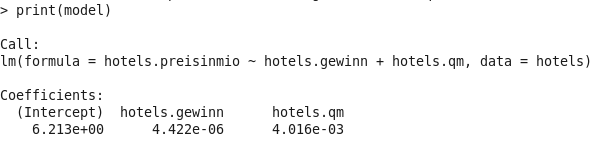
\includegraphics[width=0.70\textwidth]{pics/Hotels_model_1.png}\par\vspace{0cm}
                \caption{Ausgabe: hotels}
                \label{fig:hive5}
        \end{minipage}
\end{figure}


\item[-] multiples Rm (mRm) erstellen: hotels.preisinmio = a * hotels.gewinn + b * hotels.qm + c * hotels.stadt
\begin{lstlisting}
model <-lm(hotels.preisinmio~hotels.gewinn+hotels.qm+hotels.stadt, data = hotels)
\end{lstlisting}

\item[-] Modell Zusammenfassung ausgeben lassen (\autoref{fig:hive6})
\begin{figure}[!htb]
        \begin{minipage}{1\textwidth}
                \centering
                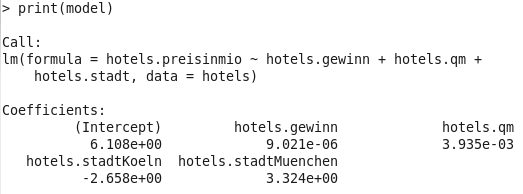
\includegraphics[width=0.70\textwidth]{pics/Hotels_model_2.png}\par\vspace{0cm}
                \caption{Ausgabe: hotels}
                \label{fig:hive6}
        \end{minipage}
\end{figure}
\item[-] Erstellen einer neuen Spalte in Autos die den Preis auf Basis des mRm (\autoref{fig:hive7}: 
\begin{lstlisting}
hotels$predicted\_2 <- predict(model, hotels)
\end{lstlisting}
\begin{figure}[!htb]
        \begin{minipage}{1\textwidth}
                \centering
                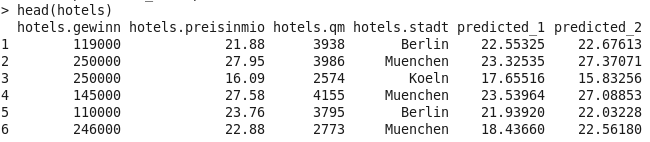
\includegraphics[width=0.70\textwidth]{pics/hotels_head.png}\par\vspace{0cm}
                \caption{Ausgabe: hotels}
                \label{fig:hive7}
        \end{minipage}
\end{figure}
\end{itemize}

\subsection*{Aufteilung der Aufgaben im Team}
Alle Aufgabenpunkte wurden gemeinsam bearbeitet.
\subsection*{Darstellung der benutzen Werkzeuge und Systeme}
\subsubsection*{Entwurfswerkzeug}
- HIVE 

\subsubsection*{Entwicklungsumgebung}
- R





\newpage


\section{14.06.2018 - ARIS}
- Definieren Sie für Ihr fiktives/reales Unternehmen folgende Diagrammtypen: Datenmodell, Geschäftsprozess, IT-Infrastruktur, Organigramm, Prozesslandschaft, BPMN, Whiteboard Beispiel, Systemlandschaft. Die Beispiele finden Sie im Elli.

\subsection{Kurzdarstellung der Aufgabenstellung}
Es sollen die grundlegenden Funktionen anhand von Diagrammen dargestellt werden.
\subsection{Lösung}
- Installation ARIS
- starten ARIS
- Diagramme für den entsprechenden Aufgabenbereich Auswählen

1. Organigramm

2. Prozesslandschaft

3. Geschäftsprozess

4. Datenmodell

5. IT-In

6.

7.

8.

\subsection{Aufteilung der Aufgaben im Team}
\subsection{Darstellung der benutzen Werkzeuge und Systeme}
\subsubsection*{Entwurfswerkzeug}
\subsubsection*{Entwicklungsumgebung}








































\end{document}


